\section{Performance Evaluation}
\label{sec:performance-evaluation}

\definecolor{npc}{RGB}{150,150,150}
\definecolor{lvpc}{RGB}{66,133,244}
\definecolor{vac}{RGB}{244,160,0}
\definecolor{metac}{RGB}{52,168,83}
\definecolor{candc}{RGB}{171,71,188}
\pgfplotsset{
    perfbar/.style={
        ybar, ymin=0, ymajorgrids, grid style={gray!25},
        axis line style={gray!60}, tick style={gray!60},
        xtick=data, xtick pos=bottom, ytick pos=left,
        ticklabel style={font=\footnotesize},
        label style={font=\footnotesize},
        legend style={at={(0.5,1.02)}, anchor=south, legend columns=-1,
                      draw=none, font=\footnotesize,
                      /tikz/every even column/.append style={column sep=6pt}},
        nodes near coords,
        every node near coord/.append style={font=\tiny},
    },
}

\subsection{Experimental Methodology}
\label{subsec:performance-methodology}

\subsubsection{Simulation Configuration and Workloads}

All experiments use gem5 MinorCPU with RISC-V syscall emulation,
an L1 data cache, an L2 cache, and the default memory-functional-unit
timing (\texttt{extraAssumedLat = 2}). NP and LVP use
\texttt{configs/research/vp\_baseline.py}, while V-ASTRA and META
are configured through \texttt{tests/astra/with\_params.py}.

The twelve workloads are stable, random base, alternating value,
V-cache miss, stable flip, V-cache flip, none, forwarding cold, mixed,
store producer, forwarding both, and forwarding flip. The first four use 100 warm-up
laps followed by 200 measured laps. The resulting counters are
consistent with this setup. For example, four chain loads per lap
produce 800 L1D read misses in the measured region.

The first four workloads share a four-load dependency chain
$P\rightarrow C\rightarrow E\rightarrow F$, in which each load supplies
the next load's address. Here $P$ is the producer load, $C$ the
dependent consumer load, and $E$ and $F$ the third and fourth loads in
the chain. Conflict stores evict the chain lines from L1D
on each lap, and the V-cache-miss variant spaces the lines 4~KiB apart
so that they share a value-cache index.
Table~\ref{tab:workload-characteristics} describes all twelve workloads.

\begin{table}[H]
    \centering
    \small
    \setlength{\tabcolsep}{4pt}
    \renewcommand{\arraystretch}{1.15}
    \caption{Workloads and what each one tests}
    \label{tab:workload-characteristics}
    \begin{tabularx}{\linewidth}{@{}>{\raggedright\arraybackslash}p{0.17\linewidth}>{\raggedright\arraybackslash}X>{\raggedright\arraybackslash}X@{}}
        \toprule
        \textbf{Workload} & \textbf{Pattern} & \textbf{What it tests} \\
        \midrule
        Stable & Addresses and values are the same every lap. &
        It is the best case for both LVP and V-ASTRA. \\
        Random base & $P$ reads a randomly chosen line, but all lines hold
        the same value. &
        LVP can predict the value, but $P$'s address is unpredictable. \\
        Alternating value & The value at $P$ changes every lap. &
        LVP cannot become confident, but V-ASTRA can still predict. \\
        V-cache miss & Chain lines map to the same value-cache entry. &
        V-ASTRA always misses, so only LVP can help. \\
        Stable flip & The value at $P$ changes every 32 laps. &
        It tests periodic LVP mispredictions and recovery. \\
        V-cache flip & It uses the V-cache-miss layout, and the value changes every
        32 laps. &
        It tests LVP recovery when V-ASTRA gives almost no benefit. \\
        None & Addresses and values are random. &
        It was meant to defeat both predictors. V-ASTRA still reduced
        cycles by 18.57\%. \\
        Forwarding cold & An older cold load stalls the pipeline before
        a dependent pair of loads. &
        It tests V-ASTRA bypass and forwarding to the dependent load. \\
        Mixed & A V-cache-miss chain is followed by a forwarding-cold
        segment. &
        LVP helps one part and V-ASTRA the other. META is faster than
        both. \\
        Store producer & An older store to a cold address precedes the stable chain. &
        It was meant to make META wait for V-ASTRA. This case did not
        occur. \\
        Forwarding both & It uses the forwarding layout with data already in the cache. &
        It tests forwarding when little latency is left to hide. The
        gain is small. \\
        Forwarding flip & It uses the forwarding layout, and the value changes every
        32 laps. &
        It tests forwarding with periodic LVP mispredictions. The gain
        is small. \\
        \bottomrule
    \end{tabularx}
\end{table}

\subsubsection{Measurement and Repetition}

The principal metric is \texttt{numCycles} in the measured region.
Only the first statistics block is used. The repeated end-of-run
block is not added. Cycle reduction relative to NP is calculated as
\[
  \text{Reduction (\%)} =
  100\,\frac{C_{\mathrm{NP}}-C_{\mathrm{mode}}}
  {C_{\mathrm{NP}}}.
\]

Each performance-sweep cell has five runs using identical executable
bytes but different output-path lengths. Results are deterministic
in almost all cells. The few differences have a spread of at most
approximately 0.15\%. These repetitions therefore check sensitivity
to output-path layout rather than provide independent samples for
statistical confidence. An additional exact run reproduced the stable
NP result.

\subsection{Standalone Predictor Comparison}
\label{subsec:standalone-predictor-performance}

Figure~\ref{tab:standalone-predictor-cycles} compares the cycle
reduction of LVP-only and V-ASTRA-only relative to NP.

\begin{figure}[H]
    \centering
    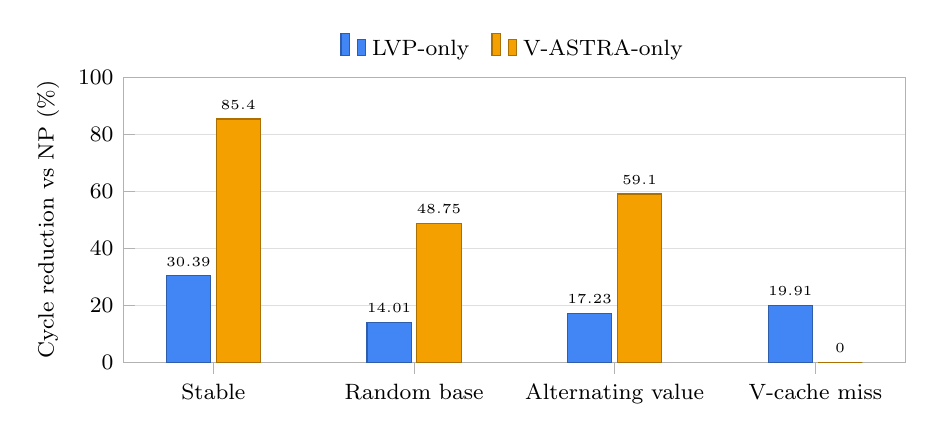
\begin{tikzpicture}
    \begin{axis}[perfbar, width=0.95\linewidth, height=5.2cm,
        bar width=16pt, ymax=100, enlarge x limits=0.15,
        ylabel={Cycle reduction vs NP (\%)},
        symbolic x coords={Stable,Random base,Alternating value,V-cache miss}]
        \addplot[fill=lvpc, draw=lvpc!70!black] coordinates
            {(Stable,30.39) (Random base,14.01) (Alternating value,17.23) (V-cache miss,19.91)};
        \addplot[fill=vac, draw=vac!70!black] coordinates
            {(Stable,85.40) (Random base,48.75) (Alternating value,59.10) (V-cache miss,0)};
        \legend{LVP-only, V-ASTRA-only}
    \end{axis}
    \end{tikzpicture}
    \caption{Cycle reduction of the standalone predictors relative to NP.
    NP takes 34,547, 35,608, 31,344, and 31,144 cycles on the four
    workloads, respectively.}
    \label{tab:standalone-predictor-cycles}
\end{figure}

V-ASTRA's benefit depends on successful value-cache hits. On the
stable workload, it produces 800 synthetic responses and eliminates
all L1D read misses. On random base, it produces 595 synthetic
responses, reducing L1D read misses from 800 to 205. On V-cache miss,
all 800 accesses miss the value-cache tags, producing no synthetic
responses and no cycle reduction. These runs have
\texttt{fwdAdmitted = 0}. The measured gains therefore come from
load bypass, not dependent-load forwarding.

Sensitivity tests with 100--800 measured laps and at least five
warm-up laps kept reductions within approximately 0.1 percentage
points of the primary results.

\subsection{META Performance}
\label{subsec:meta-performance}

The META sweeps compare NP, LVP-only, V-ASTRA-only, and META.
The main results use \texttt{metaAstraLvpLoads=off}. Figure~\ref{tab:meta-cycle-comparison}
shows the cycle reduction of each mode relative to NP.

\begin{figure}[H]
    \centering
    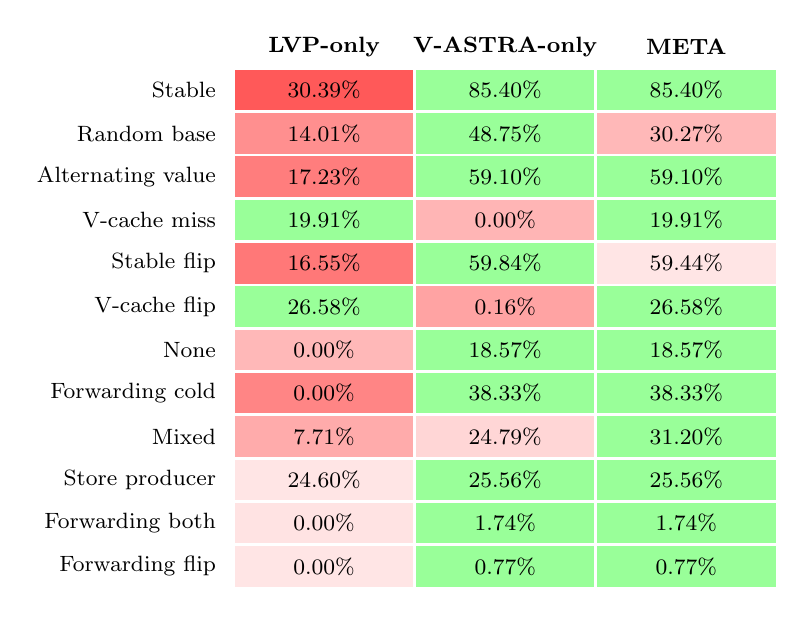
\begin{tikzpicture}[cell/.style={draw=white, line width=1pt,
        minimum width=2.30cm, minimum height=0.55cm, font=\footnotesize}]
    \node[font=\footnotesize\bfseries] at (4.15,0) {LVP-only};
    \node[font=\footnotesize\bfseries] at (6.45,0) {V-ASTRA-only};
    \node[font=\footnotesize\bfseries] at (8.75,0) {META};
    \node[anchor=east, font=\footnotesize] at (2.9,-0.55) {Stable};
    \node[cell, fill=red!65] at (4.15,-0.55) {30.39\%};
    \node[cell, fill=green!40] at (6.45,-0.55) {85.40\%};
    \node[cell, fill=green!40] at (8.75,-0.55) {85.40\%};
    \node[anchor=east, font=\footnotesize] at (2.9,-1.10) {Random base};
    \node[cell, fill=red!44] at (4.15,-1.10) {14.01\%};
    \node[cell, fill=green!40] at (6.45,-1.10) {48.75\%};
    \node[cell, fill=red!28] at (8.75,-1.10) {30.27\%};
    \node[anchor=east, font=\footnotesize] at (2.9,-1.65) {Alternating value};
    \node[cell, fill=red!51] at (4.15,-1.65) {17.23\%};
    \node[cell, fill=green!40] at (6.45,-1.65) {59.10\%};
    \node[cell, fill=green!40] at (8.75,-1.65) {59.10\%};
    \node[anchor=east, font=\footnotesize] at (2.9,-2.20) {V-cache miss};
    \node[cell, fill=green!40] at (4.15,-2.20) {19.91\%};
    \node[cell, fill=red!29] at (6.45,-2.20) {0.00\%};
    \node[cell, fill=green!40] at (8.75,-2.20) {19.91\%};
    \node[anchor=east, font=\footnotesize] at (2.9,-2.75) {Stable flip};
    \node[cell, fill=red!53] at (4.15,-2.75) {16.55\%};
    \node[cell, fill=green!40] at (6.45,-2.75) {59.84\%};
    \node[cell, fill=red!10] at (8.75,-2.75) {59.44\%};
    \node[anchor=east, font=\footnotesize] at (2.9,-3.30) {V-cache flip};
    \node[cell, fill=green!40] at (4.15,-3.30) {26.58\%};
    \node[cell, fill=red!36] at (6.45,-3.30) {0.16\%};
    \node[cell, fill=green!40] at (8.75,-3.30) {26.58\%};
    \node[anchor=east, font=\footnotesize] at (2.9,-3.85) {None};
    \node[cell, fill=red!28] at (4.15,-3.85) {0.00\%};
    \node[cell, fill=green!40] at (6.45,-3.85) {18.57\%};
    \node[cell, fill=green!40] at (8.75,-3.85) {18.57\%};
    \node[anchor=east, font=\footnotesize] at (2.9,-4.40) {Forwarding cold};
    \node[cell, fill=red!48] at (4.15,-4.40) {0.00\%};
    \node[cell, fill=green!40] at (6.45,-4.40) {38.33\%};
    \node[cell, fill=green!40] at (8.75,-4.40) {38.33\%};
    \node[anchor=east, font=\footnotesize] at (2.9,-4.95) {Mixed};
    \node[cell, fill=red!33] at (4.15,-4.95) {7.71\%};
    \node[cell, fill=red!16] at (6.45,-4.95) {24.79\%};
    \node[cell, fill=green!40] at (8.75,-4.95) {31.20\%};
    \node[anchor=east, font=\footnotesize] at (2.9,-5.50) {Store producer};
    \node[cell, fill=red!10] at (4.15,-5.50) {24.60\%};
    \node[cell, fill=green!40] at (6.45,-5.50) {25.56\%};
    \node[cell, fill=green!40] at (8.75,-5.50) {25.56\%};
    \node[anchor=east, font=\footnotesize] at (2.9,-6.05) {Forwarding both};
    \node[cell, fill=red!11] at (4.15,-6.05) {0.00\%};
    \node[cell, fill=green!40] at (6.45,-6.05) {1.74\%};
    \node[cell, fill=green!40] at (8.75,-6.05) {1.74\%};
    \node[anchor=east, font=\footnotesize] at (2.9,-6.60) {Forwarding flip};
    \node[cell, fill=red!10] at (4.15,-6.60) {0.00\%};
    \node[cell, fill=green!40] at (6.45,-6.60) {0.77\%};
    \node[cell, fill=green!40] at (8.75,-6.60) {0.77\%};
    \end{tikzpicture}
    \caption{Cycle reduction relative to NP for LVP-only, V-ASTRA-only,
    and META (\texttt{metaAstraLvpLoads=off}). Green marks the largest
    reduction for each workload. Red shading grows with the gap, in
    percentage points, to that largest reduction.}
    \label{tab:meta-cycle-comparison}
\end{figure}

META matches the better standalone predictor on nine of the twelve
workloads and improves on both for mixed, reducing cycles by
31.20\% relative to NP. However, it underperforms V-ASTRA-only on
random base (24,828 versus 18,249 cycles) and
stable flip (13,039 versus 12,912 cycles). Thus, combining
predictors does not guarantee the best result on every workload.
The performance results alone do not establish the cause of each
difference. The random-base case is examined separately below.

\subsection{Provisional-Base Modes on the Random-Base Workload}
\label{subsec:provisional-base-performance}

The \texttt{metaAstraLvpLoads} parameter was evaluated in
\texttt{off}, \texttt{train}, and \texttt{candidate} modes on the
random-base workload. Figure~\ref{tab:randbase-mode-cycles} shows
the resulting cycle reductions and L1D read misses.

\begin{figure}[H]
    \centering
    \pgfplotsset{rbmode/.style={perfbar, width=0.52\linewidth, height=5.4cm,
        bar width=13pt, enlarge x limits=0.13,
        symbolic x coords={NP,V-ASTRA,off,train,candidate},
        xticklabels={No pred.,V-ASTRA,META off,META train,META cand.},
        xticklabel style={rotate=35, anchor=north east, font=\footnotesize}}}
    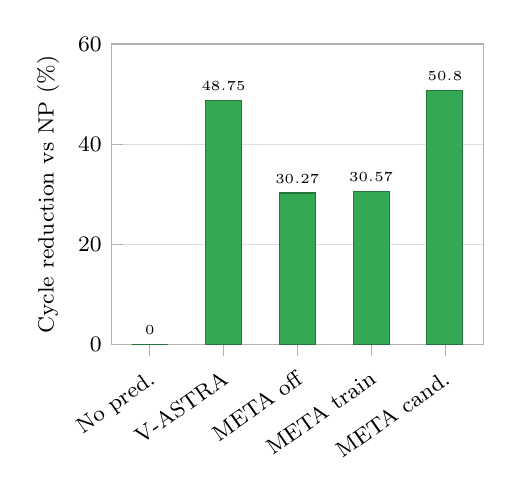
\begin{tikzpicture}
    \begin{axis}[rbmode, ymax=60, ylabel={Cycle reduction vs NP (\%)},
        nodes near coords={\pgfmathprintnumber[fixed,precision=2]{\pgfplotspointmeta}}]
        \addplot[fill=metac, draw=metac!70!black] coordinates
            {(NP,0) (V-ASTRA,48.75) (off,30.27) (train,30.57) (candidate,50.80)};
    \end{axis}
    \end{tikzpicture}\hfill
    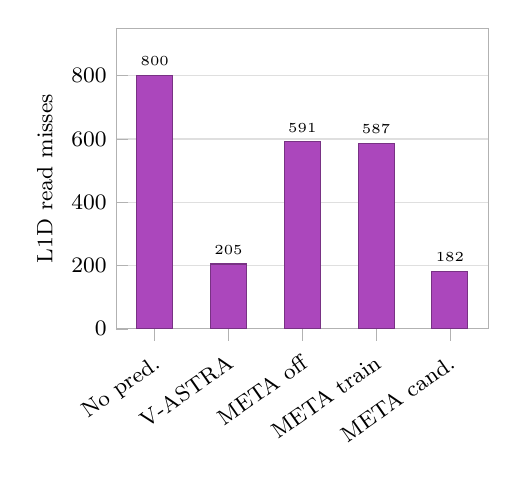
\begin{tikzpicture}
    \begin{axis}[rbmode, ymax=950, ylabel={L1D read misses}]
        \addplot[fill=candc, draw=candc!70!black] coordinates
            {(NP,800) (V-ASTRA,205) (off,591) (train,587) (candidate,182)};
    \end{axis}
    \end{tikzpicture}
    \caption{Random-base cycle reduction relative to NP (left) and L1D
    read misses (right) across provisional-base modes.}
    \label{tab:randbase-mode-cycles}
\end{figure}

Figure~\ref{tab:randbase-mode-events} shows the corresponding event
counts. The candidate count is reported by
\texttt{vastra.candidates}. In this experiment, it equals the number
of synthetic responses.

\begin{figure}[H]
    \centering
    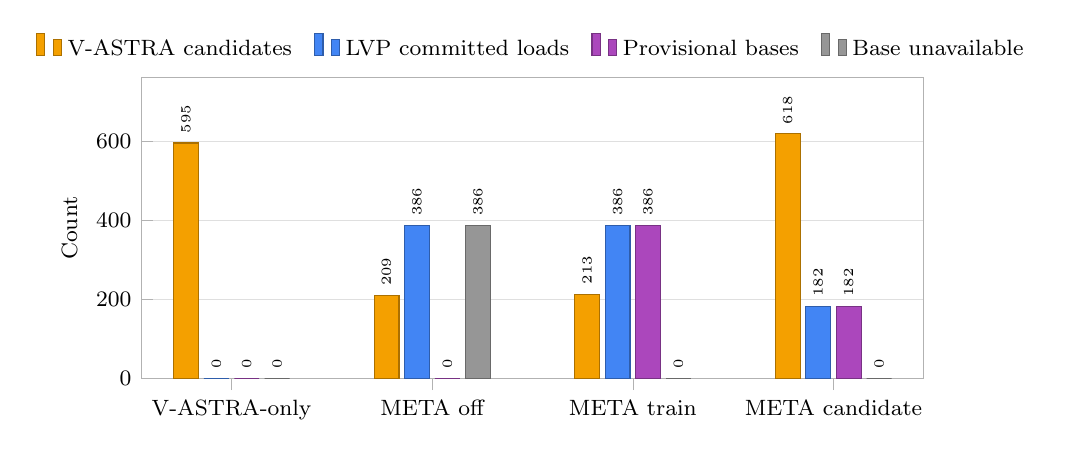
\begin{tikzpicture}
    \begin{axis}[perfbar, width=0.95\linewidth, height=5.4cm,
        bar width=9pt, ymax=760, enlarge x limits=0.15,
        every node near coord/.append style={font=\tiny, rotate=90, anchor=west},
        ylabel={Count},
        symbolic x coords={V-ASTRA-only,META off,META train,META candidate}]
        \addplot[fill=vac, draw=vac!70!black] coordinates
            {(V-ASTRA-only,595) (META off,209) (META train,213) (META candidate,618)};
        \addplot[fill=lvpc, draw=lvpc!70!black] coordinates
            {(V-ASTRA-only,0) (META off,386) (META train,386) (META candidate,182)};
        \addplot[fill=candc, draw=candc!70!black] coordinates
            {(V-ASTRA-only,0) (META off,0) (META train,386) (META candidate,182)};
        \addplot[fill=npc, draw=npc!70!black] coordinates
            {(V-ASTRA-only,0) (META off,386) (META train,0) (META candidate,0)};
        \legend{V-ASTRA candidates, LVP committed loads,
                Provisional bases, Base unavailable}
    \end{axis}
    \end{tikzpicture}
    \caption{Random-base event counts. Every provisional base was
    validated and none was dropped. V-ASTRA-only has no LVP.}
    \label{tab:randbase-mode-events}
\end{figure}

Train mode changes the cycle count by only 106 cycles relative to
off (24,722 versus 24,828). Candidate mode reduces cycles by 7,310
(29.4\%) relative to off and by 731 relative to V-ASTRA-only. It
also reduces L1D read misses from 591 to 182 and increases synthetic
responses from 209 to 618. The number of committed LVP-speculated
loads falls from 386 in off and train to 182 in candidate mode.

These counters are consistent with candidate mode restoring
V-ASTRA opportunities for some LVP-served loads. However, they do
not establish how much of the cycle reduction is caused by individual
additional bypasses. Candidate counts alone are also not a reliable
indicator of performance: on mixed, candidates increase from
390 to 988 while synthetic responses remain at 191 and cycles do not
change. On V-cache miss, candidates increase from 200 to 800, but
no synthetic responses occur and cycles remain unchanged.

The random-base experiment was repeated after the alignment retry
fix, with one run per mode. The off, train, and candidate cycle counts
exactly reproduced the five-run results.

\subsection{Performance of Dependency-Handling Designs}
\label{subsec:dependency-performance}

The performance harness uses the default memory-FU timing
(\texttt{extraAssumedLat = 2}), under which Design~A's scoreboard
release is inactive.

Design~B forwarding is enabled in the V-ASTRA performance mode, but
no V-ASTRA-without-forwarding control is available. Its contribution
therefore cannot be isolated. Figure~\ref{tab:forwarding-performance}
reports the combined configuration relative to NP. Forwarded
consumer counts are from \texttt{vastra.fwdAdmitted} and represent
admitted consumers, not committed instructions.

\begin{figure}[H]
    \centering
    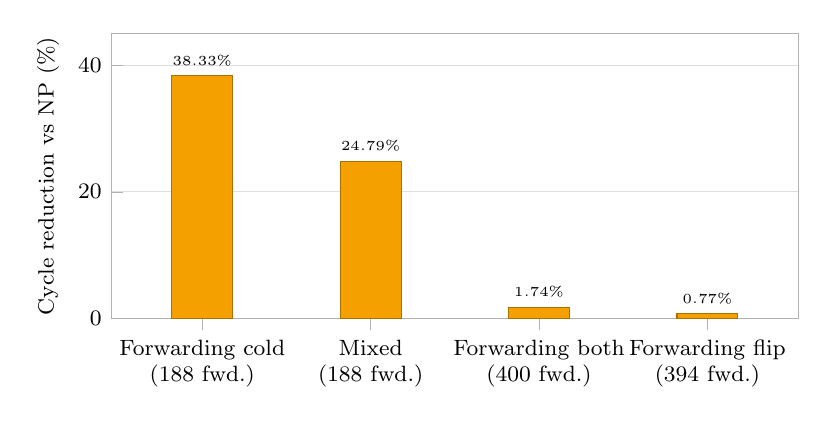
\begin{tikzpicture}
    \begin{axis}[perfbar, width=0.85\linewidth, height=5.2cm,
        bar width=22pt, ymax=45, enlarge x limits=0.18,
        ylabel={Cycle reduction vs NP (\%)},
        symbolic x coords={fc,mx,fb,ff},
        xticklabels={{Forwarding cold\\(188 fwd.)},{Mixed\\(188 fwd.)},
                     {Forwarding both\\(400 fwd.)},{Forwarding flip\\(394 fwd.)}},
        xticklabel style={align=center},
        nodes near coords={\pgfmathprintnumber[fixed,precision=2]{\pgfplotspointmeta}\%}]
        \addplot[fill=vac, draw=vac!70!black] coordinates
            {(fc,38.33) (mx,24.79) (fb,1.74) (ff,0.77)};
    \end{axis}
    \end{tikzpicture}
    \caption{Cycle reduction of V-ASTRA (with forwarding) relative to NP
    on the forwarding workloads. The number of forwarded consumers
    (\texttt{vastra.fwdAdmitted}) is given under each workload.}
    \label{tab:forwarding-performance}
\end{figure}

Forwarding cold reduces cycles by 38.33\% while L1D misses remain
unchanged at 400, despite 191 synthetic responses. This is consistent
with a benefit from overlap, although the measurements do not isolate
its contribution. The gains on forwarding both and forwarding flip
are smaller (1.74\% and 0.77\%), with path-padding spreads of
approximately 0.059\% and 0.152\%, respectively.

\subsection{Threats to Validity and Interpretation}
\label{subsec:performance-limitations}

The results are deterministic microbenchmark measurements on a single
MinorCPU, cache, and memory configuration. They do not represent
application-level speedups. The repeated runs check sensitivity to
output-path layout only and are not independent statistical samples.
Design~A was not measured under the default timing, and the
contribution of Design~B cannot be separated from V-ASTRA. Small
effects close to the observed layout variation should therefore be
interpreted with caution.

Overall, the cycle reductions are substantial but depend on the
workload. META improves on both standalone predictors on mixed, but is
slower than V-ASTRA-only on random base and stable flip. Candidate mode
gives a large improvement on random base, but its broader benefit is not
established by these workloads.
